\documentclass{beamer}
\usepackage{listings}
\lstset{
%language=C,
frame=single, 
breaklines=true,
columns=fullflexible
}
\usepackage{subcaption}
\usepackage{url}
\usepackage{amsmath}

\usepackage{amsthm}

\usepackage{tikz}
\usepackage{graphicx}
\usepackage{tkz-euclide} % loads  TikZ and tkz-base
%\usetkzobj{all}
\usetikzlibrary{calc,math}
\usepackage{float}

\newcommand\norm[1]{\left\lVert#1\right\rVert}
\renewcommand{\vec}[1]{\mathbf{#1}}
\newcommand{\R}{\mathbb{R}}
\newcommand{\C}{\mathbb{C}}
\providecommand{\brak}[1]{\ensuremath{\left(#1\right)}}
\providecommand{\abs}[1]{\vert#1\vert}
\providecommand{\fourier}{\overset{\mathcal{F}}{ \rightleftharpoons}}
\newcommand{\myvec}[1]{\ensuremath{\begin{pmatrix}#1\end{pmatrix}}}
\providecommand{\mean}[1]{E[ #1 ]}
\providecommand{\sbrak}[1]{\ensuremath{{}\left[#1\right]}}
\providecommand{\cbrak}[1]{\ensuremath{\left\{#1\right\}}}
\usepackage[export]{adjustbox}
\usepackage[utf8]{inputenc}
\usepackage{amsmath}
\usetheme{Boadilla}
\title{A New Probabilistic Gradient Descent Bit Flipping Decoder for LDPC Codes}
\author{Adepu Adarsh Sai}
\institute{IITH(AI)}
\date{\today}
\begin{document}

\begin{frame}
\titlepage
\end{frame}
\begin{frame}{Exclusive-OR operation(XOR)}
\begin{block}{XOR operation}
 If number of 1s at it inputs is odd then the output is 1\\
 If number of 1s at it inputs is even then the output is 0
 \end{block}
 \begin{figure}[h]
    \centering
    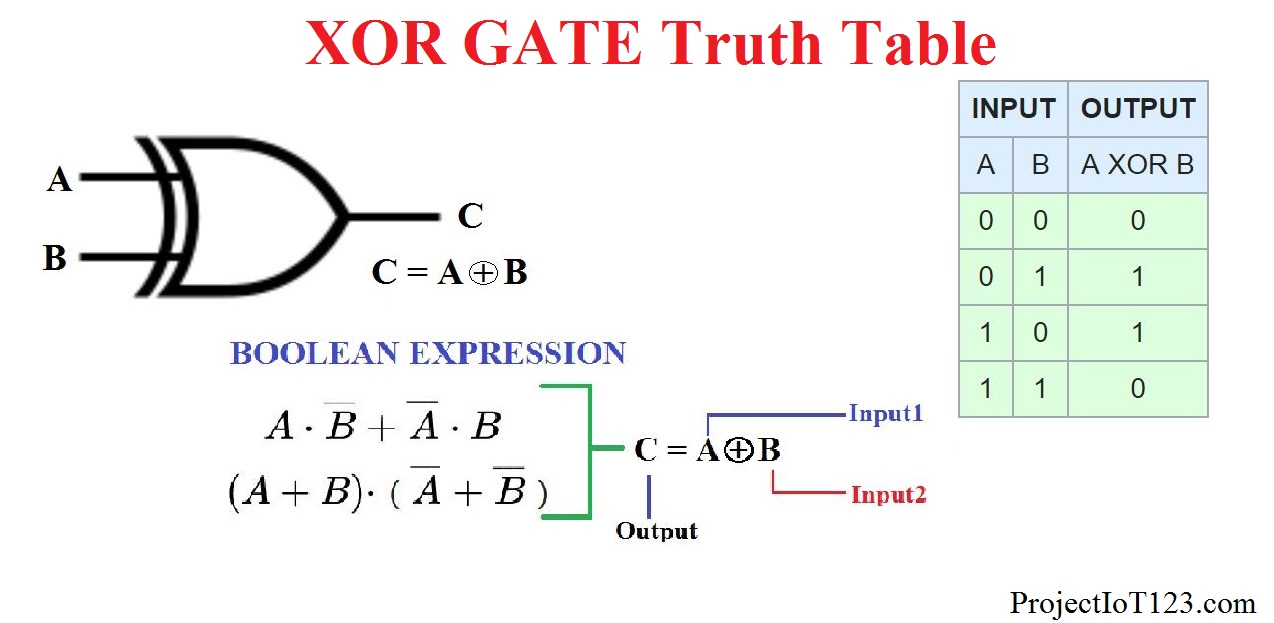
\includegraphics[width=0.8\textwidth]{XOR.jpg}
\end{figure}    
\end{frame}
\begin{frame}{Binary Symmetric Channel $\brak{BSC_{p}}$}
$\bullet$ It is a communications channel model used in   coding theory and information theory.\\
$\bullet$ A transmitter wishes to send a bit(0 or 1). and the receiver will receive a bit.\\
$\bullet$ The bit will be flipped with a "crossover probability" of p. and otherwise is received correctly.
\begin{figure}[h]
    \centering
    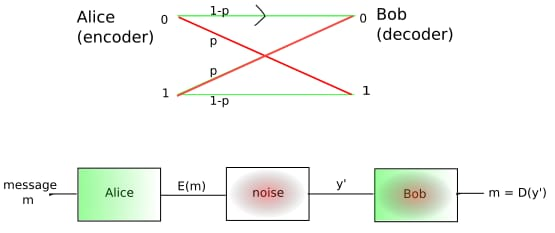
\includegraphics[width=0.8\textwidth]{BSC.jpeg}
\end{figure}
\end{frame}
\begin{frame}{Low-Density Parity-Check code(LDPC)}
    \begin{block}{LDPC}
    A low-density parity-check code is a linear error correcting code, a method of transmitting a message over a noisy transmission channel.
    \end{block}
    We can represent an LDPC code graphically, for example
    \begin{figure}[h]
    \centering
    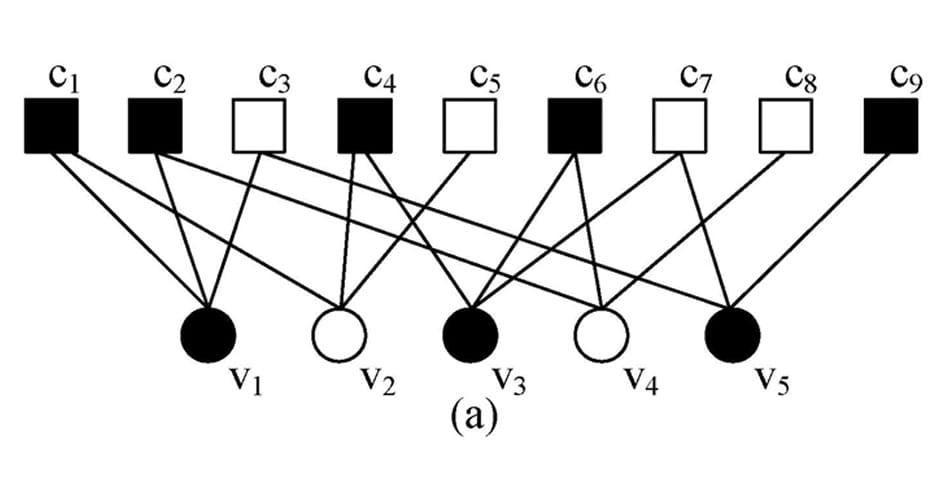
\includegraphics[width=0.5\textwidth]{LDPC code.jpeg}
\end{figure}
%Its parity-check matrix $\textbf{H}$ is given by
\end{frame}
 \begin{frame}{Parity-Check matrix}
 \begin{block}{Parity-check matrix}
 In coding theory, a parity-check matrix $\textbf{H}_{(M\times N)}$ of a linear block code C is a matrix which describes the linear relations that the components of a codeword must satisfy.
 \end{block}
 $\bullet$ Each row of $\textbf{H}$ corresponds to a parity check equation which is represented by a Check Node(CN)\\
  $\bullet$ Each column represents a codeword symbol which is denoted by a Variable Node(VN)\\
  $\bullet$ Code rate $R=1-\frac{M}{N}$\\
  $\bullet$ A length-N binary vector $\textbf{u}$ is a codeword if and only if $\textbf{u}\odot\textbf{H}^{\top}=0$\\
  $\bullet$ $\textsc{N}_c(i)$ is the set of VNs connected to i-th CN, i.e $\textsc{N}_c(i)=\cbrak{j|h_{i.j}=1}$.Similarly we can define $\textsc{N}_v(j)$.\\
  $\bullet$ Degree of j-th VN,$d_v^j=|\textsc{N}_v(j)|$.Similarly we can define $d_c^i$\\
 $\bullet$ $i\in \cbrak{0,1,..,M-1}$ and $j\in \cbrak{0,1,..,N-1}$\\
\textbf{NOTE}: $\odot$ is symbol of mod 2 multiplication.
\end{frame}

%\begin{frame}{}
  %%\begin{align}
      %\textbf{H}=\myvec{1&1 &0 &0 &0\\  
       %                 1&0 &0 &1 &0\\
      %                  1&0 &0 &0 &1\\  
      %                  0&1 &1 &0 &0\\
      %                  0&1 &0 &0 &0\\  
       %                 0&0 &1 &1 &0\\  
       %                 0&0 &1 &0 &1\\  
       %                 0&0 &0 &1 &0\\  
       %                 0&0 &0 &0 &1  }
 % \end{align}
 
%\end{frame}
\begin{frame}{Inversion Function}
Inversion function for BSC channel is given by
 \begin{align}
     \Lambda_j=c_j\oplus r_j +\sum_{i\in \textsc{N}_v(j)}s_i
 \end{align}
 where\\
 $\bullet$ $j\in \cbrak{0,1,..,N-1}$\\
 $\bullet$ $\textbf{c}$ is estimated codeword(N$\times$ 1)\\
 $\bullet$ $\textbf{r}$ is received codeword(N$\times $1)\\
 $\bullet$ $\textbf{s}$ is syndrome vector(M$\times$1)
 \begin{align}
     s_i=\oplus_{j\in \textsc{N}_c(i)} c_j
 \end{align}
 $\bullet$ $\oplus$ represents bit-wise XOR operation\\
 The value of the inversion function is called energy value of the respective bit.
 \end{frame}
 \begin{frame}{Hierarchy of Bit Flipping decoders}
 \begin{center}
     
 
\framebox[\width]{\textcolor{red}{T-PGDBF}} \par
$\uparrow$\\
\framebox[\width]{\textcolor{blue}{PGDBF}} \par
$\uparrow$\\
\framebox[\width]{\textcolor{green}{GDBF}} \par
$\uparrow$\\
\framebox[\width]{\textcolor{yellow}{BF}}\\
\end{center} 
 
\textcolor{yellow}{BF} algorithm:\\
$\bullet$ Energy value of each bit is calculated from inversion function.\\
$\bullet$ If the energy value is above certain value then the bit is flipped.\\
$\bullet$ The process is iterated.\\
\textcolor{green}{GDBF} algorithm:\\
$\bullet$ Energy value of each bit is calculated from inversion function.\\
$\bullet$ The bits which have the maximum energy value are flipped.\\
\end{frame}
\begin{frame}{}
  \textcolor{blue}{PGDBF} algorithm:\\
  $\bullet$ Compared to the GDBF algorithm, only a randomly selected subset of bits which have the maximum energy value are flipped in the PGDBF algorithm.
  \begin{figure}[h]
    \centering
    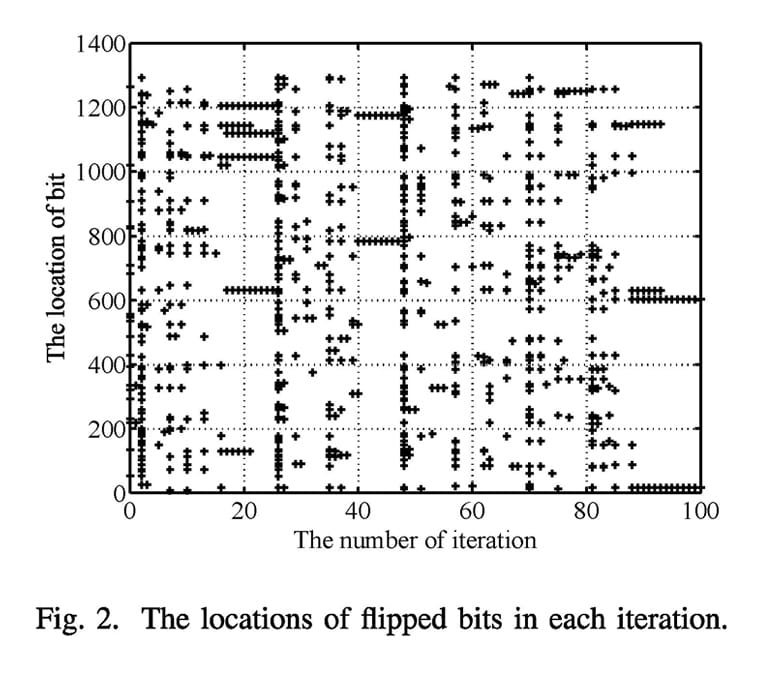
\includegraphics[width=0.5\textwidth]{trap.jpeg}
\end{figure}
\centering
A $d_v=4$, $d_c=8$, $R=0.5$, $N=1296(dv4R050N1296)$ code is used and $T_{max}=300$.
\end{frame}
\begin{frame}{T-PGDBF algorithm}
  $\bullet$ From Fig-2 it can be seen that some bits are flipped repeatedly in several iterations,which are called trapping sets.\\
  \textcolor{red}{T-PGDBF} algorithm:\\
  $\bullet$ So a tabu-list is defined and the  bits which are flipped in the current iteration
will be added to this list.\\
$\bullet$ Only the bits which are not in the
tabu-list and have the maximum energy value are flipped with probability $p_o$.
   
\end{frame}
\begin{frame}{T-PGDBF algorithm}
  \begin{figure}[h]
    \centering
    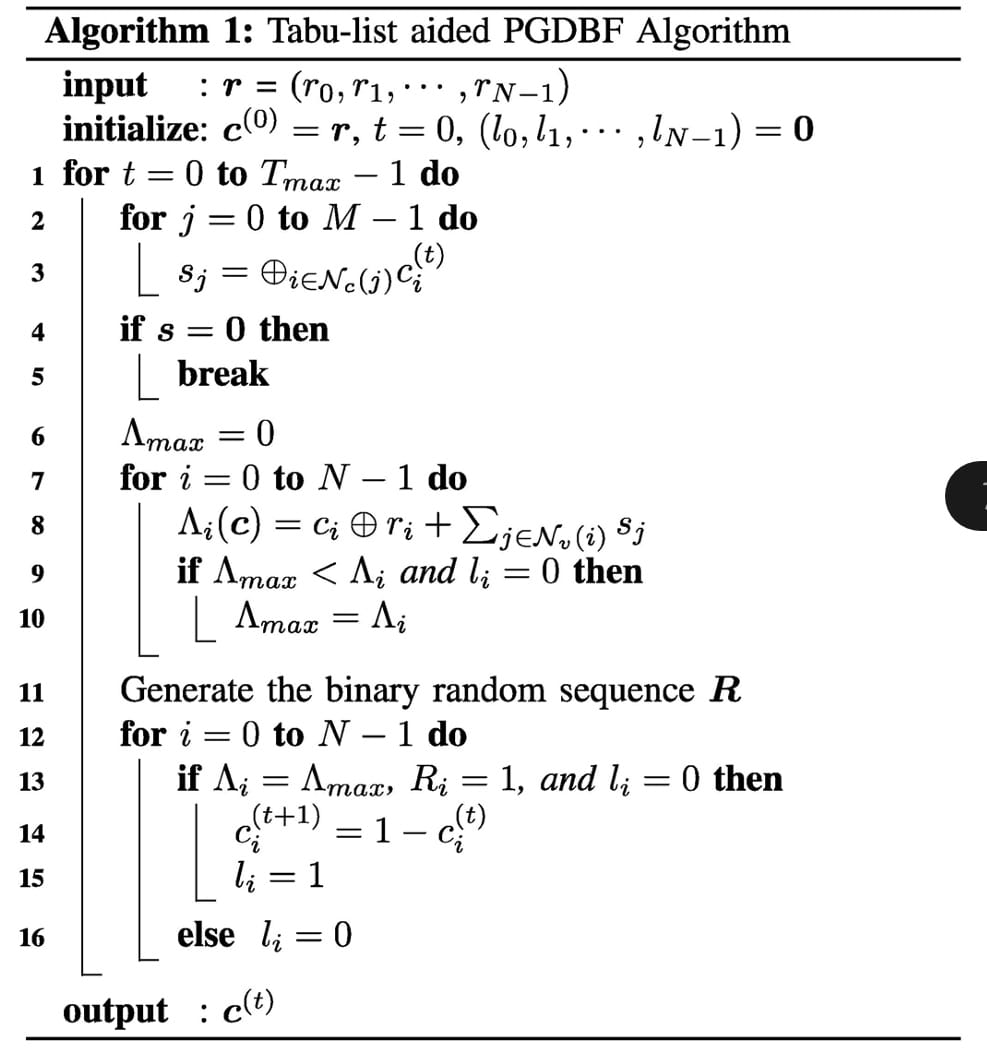
\includegraphics[width=0.6\textwidth]{T-PGDBF Alg.jpeg}
\end{figure}  
\end{frame}
\begin{frame}{}
    $\bullet$ \textbf{r} is received codeword.\\
    $\bullet$ $c^{(t)}$ denotes the estimated codeword  in the t-th iteration.\\
    $\bullet$ $l_i$ indicates whether the i-th bit is in tabu-list or not.\\
    $\bullet$ M = Number of CNs.\\
    $\bullet$ N = Number of VNs.\\
    $\bullet$ \textbf{s} is syndrome vector.\\
    $\bullet$ $\Lambda_i=$ energy value of i-th bit.\\
    $\bullet$ R is the random sequence and $Pr\cbrak{R_i=1}=p_o$ 
\end{frame}
\begin{frame}{Simulation Results}
    \begin{figure}[h]
    \centering
    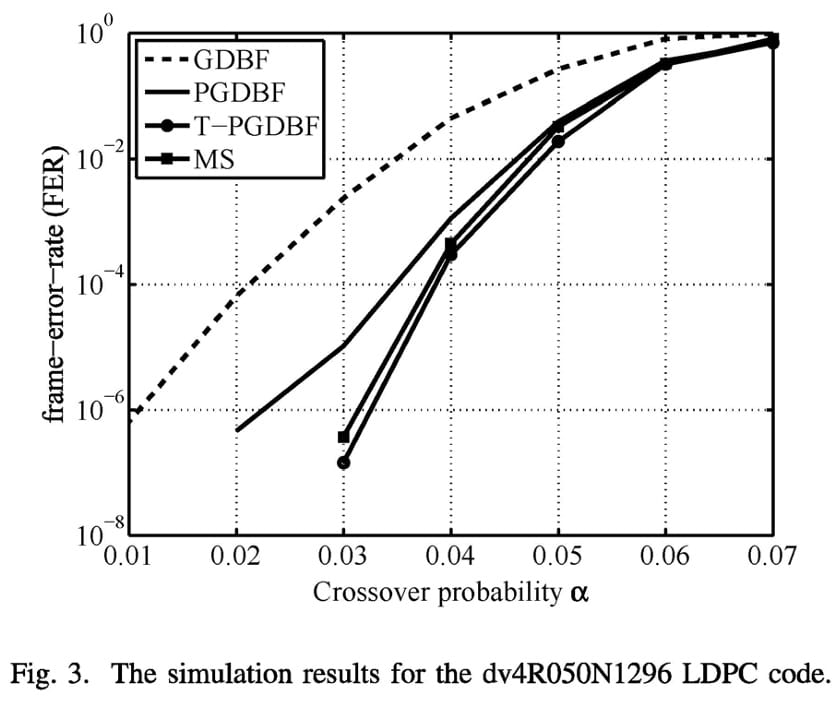
\includegraphics[width=0.6\textwidth]{Simulation.jpeg}
\end{figure}
\centering $T_{max}$ is set to 20 for MS algorithm,otherwise $T_{max}=300$, $p_o=0.9$ 
\end{frame}
\begin{frame}{Hardware Architecture}
    \begin{figure}[h]
    \centering
    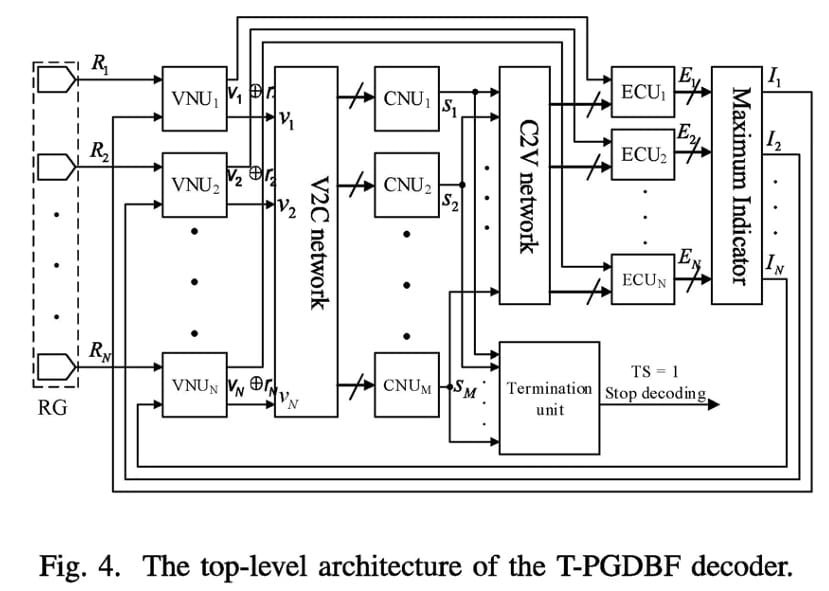
\includegraphics[width=0.6\textwidth]{Hardware.jpeg}
\end{figure}
$\bullet$ At the initializaion of the decoding, \textbf{r} is assigned to the estimated codeword \textbf{v} in VN units(VNUs).\\
$\bullet$ M CN units(CNUs) are used to calculated the syndrome vector \textbf{s}.\\
 
\end{frame}
\begin{frame}{}
$\bullet$ The energy values are calculated in N ECUs and the maximum indicator produces the indicator value $I_i$ of each bit.\\
$\bullet$ For the bits which have maximum energy value, $I_i=1$, otherwise $I_i=0$.\\
$\bullet$ The random sequence R is pre-generated and cyclically shifted once in each iteration.\\
$\bullet$ In each iteration, the termination unit will perform an OR operation among the whole syndrome vector to verify whether the current estimated codeword is valid or not.\\
$\bullet$ When the valid codeword is obtained or the maximum number of iterations is reached, TS=1
and the decoder is stopped.    
\end{frame}
\begin{frame}{Additional Architecture}
    \begin{figure}[h]
    \centering
    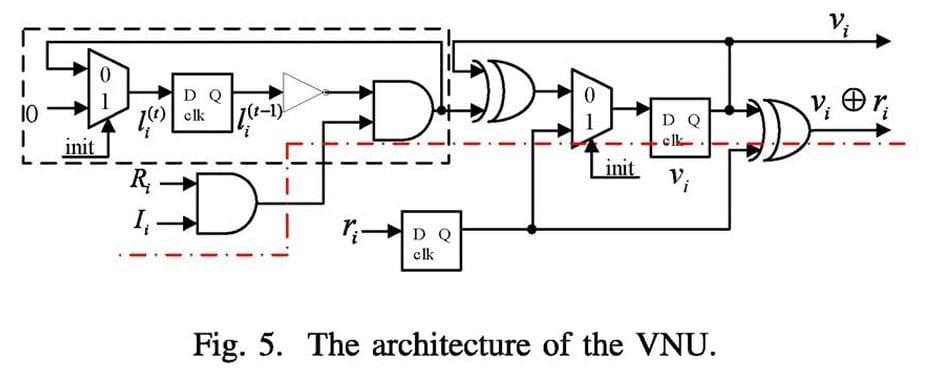
\includegraphics[width=1\textwidth]{VNU.jpeg}
\end{figure}
$\bullet$ The signal \textit{init} is only triggered once to initialize $l_i$ and $v_i$.\\
\end{frame}
\begin{frame}{}
   \begin{figure}[h]
    \centering
    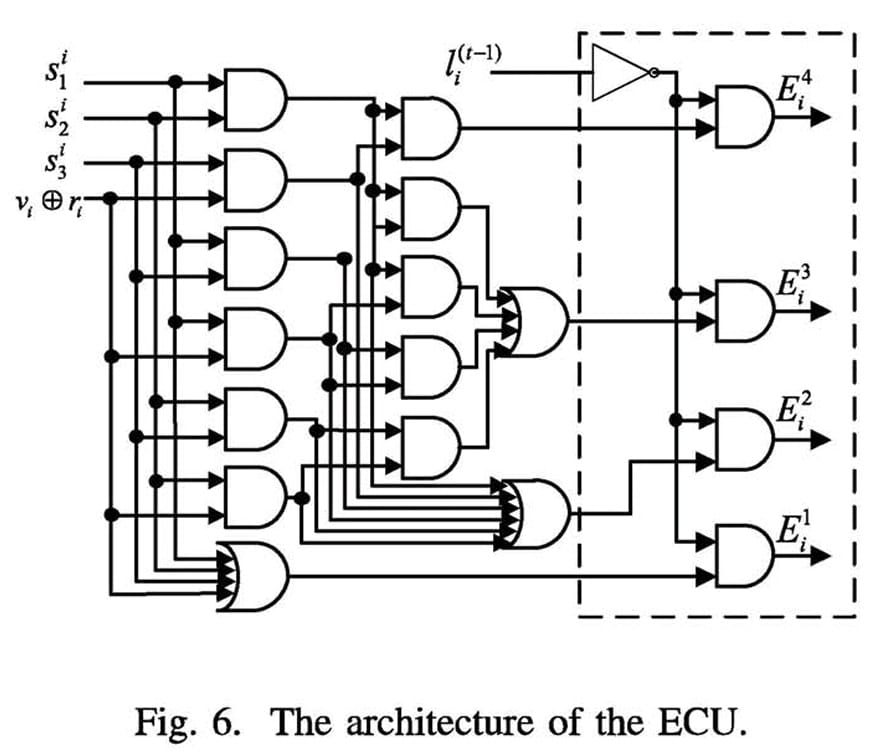
\includegraphics[width=0.6\textwidth]{ECU.jpeg}
\end{figure} 
$\bullet$ Fig-6 shows the ECU which is designed for the code with $d_v=3$. $s_1^i,s_2^i,s_3^i$ are the syndromes connected to the i-th VN.\\
$\bullet$ The energy value is expressed in one-hot format. i.e $E_i^{d_v+1}...E_i^2E_i^1$ where $E_i^k=1$ if and only if $E_i=k$.
\end{frame}
\begin{frame}{Synthesis and comparison results}
  \begin{figure}[h]
    \centering
    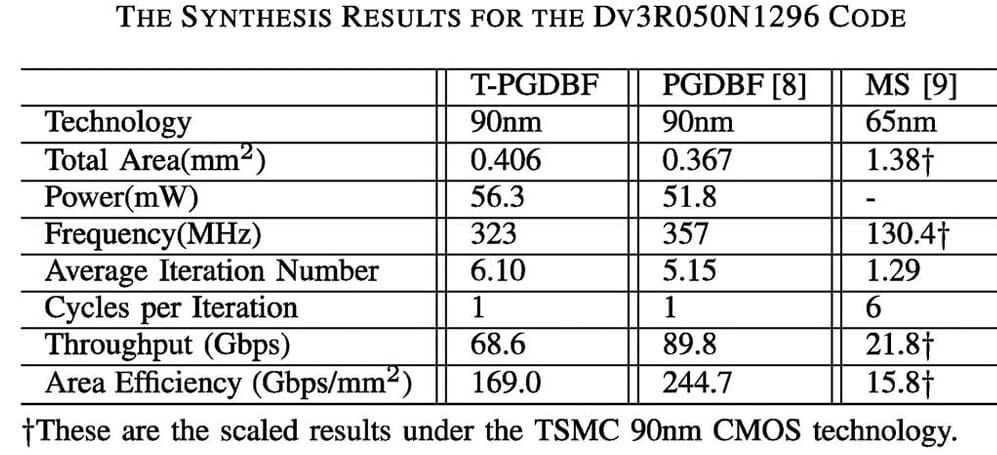
\includegraphics[width=0.6\textwidth]{Comparison.jpeg}
\end{figure}
$\bullet$ Compared to the PGDBF decoder, the T-PGDBF decoder requires $10.6\%$ extra area and $8.7\%$ extra power.\\
$\bullet$ T-PGDBF operates at lower frequency.\\
$\bullet$ Therefore, the proposed T-PGDBF algorithm has greater potential in practical applications due to its high-performance and high-throughput property.
\end{frame}
\end{document}